\documentclass{standalone}
\usepackage{tikz}
\usetikzlibrary{patterns, positioning}
\usepackage[sfdefault]{ClearSans} %% option 'sfdefault' activates Clear Sans as the default text font
\usepackage[T1]{fontenc}

\begin{document}
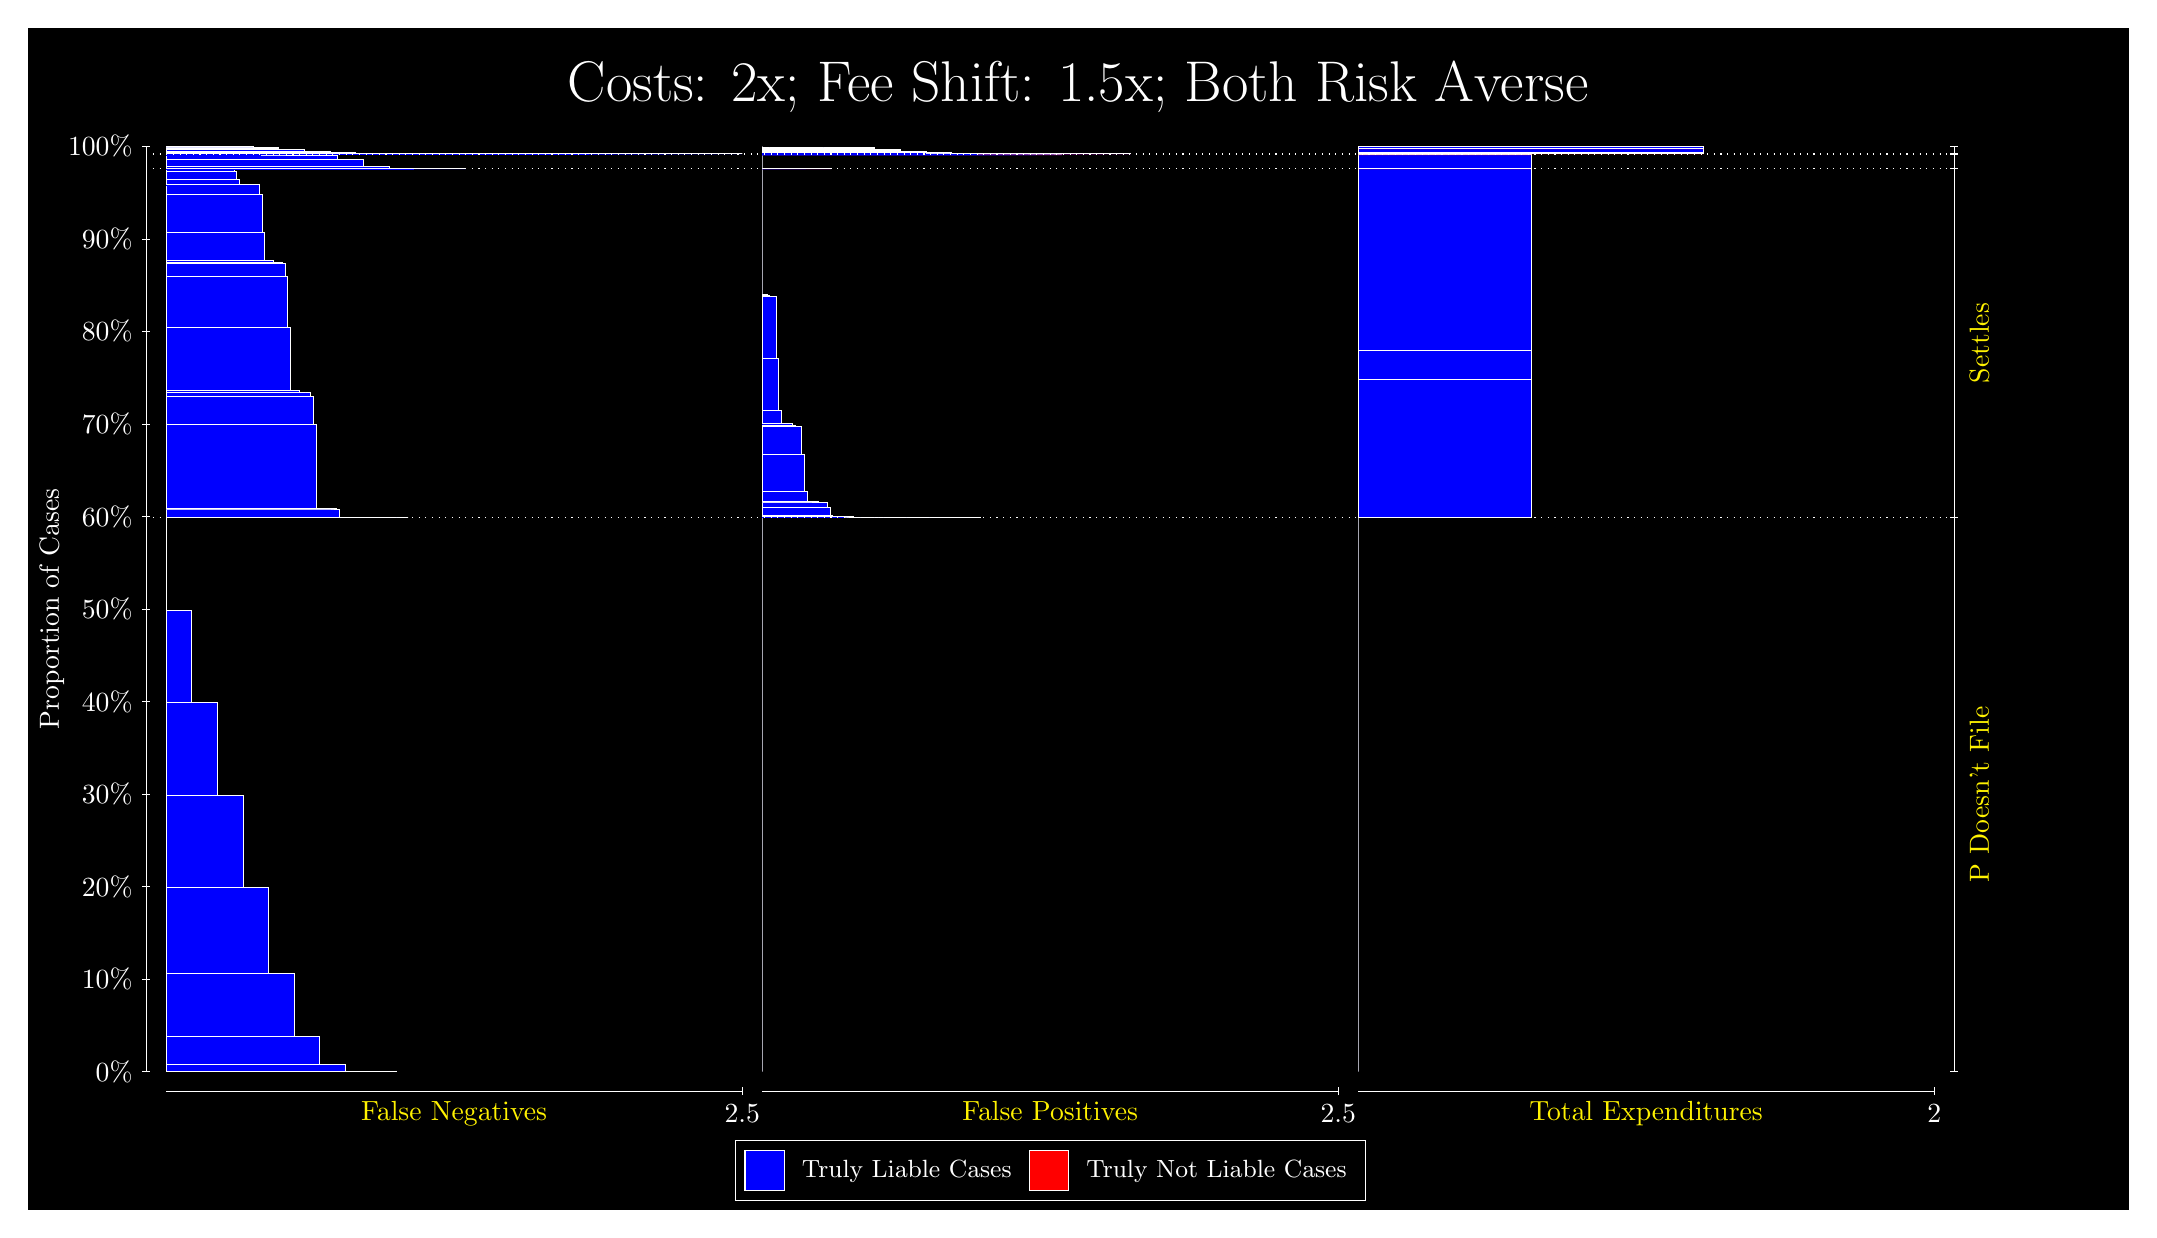
\begin{tikzpicture}
\draw[fill=black] (0,0) rectangle (26.667,15);
\draw[text=white] (0,13.5) rectangle (26.667,15) node[midway] {\huge Costs: 2x; Fee Shift: 1.5x; Both Risk Averse};
\draw[white, very thin] (1.5,1.75) -- (1.5,13.5);
\node[rotate=90, text=white, anchor=center] at (0.3, 7.625) {Proportion of Cases};
\draw[white, very thin] (1.45,1.75) -- (1.55,1.75);
\node[text=white, anchor=east] at (1.45, 1.75) {0\%};
\draw[white, very thin] (1.45,2.925) -- (1.55,2.925);
\node[text=white, anchor=east] at (1.45, 2.925) {10\%};
\draw[white, very thin] (1.45,4.1) -- (1.55,4.1);
\node[text=white, anchor=east] at (1.45, 4.1) {20\%};
\draw[white, very thin] (1.45,5.275) -- (1.55,5.275);
\node[text=white, anchor=east] at (1.45, 5.275) {30\%};
\draw[white, very thin] (1.45,6.45) -- (1.55,6.45);
\node[text=white, anchor=east] at (1.45, 6.45) {40\%};
\draw[white, very thin] (1.45,7.625) -- (1.55,7.625);
\node[text=white, anchor=east] at (1.45, 7.625) {50\%};
\draw[white, very thin] (1.45,8.8) -- (1.55,8.8);
\node[text=white, anchor=east] at (1.45, 8.8) {60\%};
\draw[white, very thin] (1.45,9.975) -- (1.55,9.975);
\node[text=white, anchor=east] at (1.45, 9.975) {70\%};
\draw[white, very thin] (1.45,11.15) -- (1.55,11.15);
\node[text=white, anchor=east] at (1.45, 11.15) {80\%};
\draw[white, very thin] (1.45,12.325) -- (1.55,12.325);
\node[text=white, anchor=east] at (1.45, 12.325) {90\%};
\draw[white, very thin] (1.45,13.5) -- (1.55,13.5);
\node[text=white, anchor=east] at (1.45, 13.5) {100\%};

\draw[white, very thin] (24.457,1.75) -- (24.457,13.5);
\draw[white, very thin] (24.407,1.75) -- (24.507,1.75);
\node[anchor=west] at (24.407, 1.75) {};
\draw[white, very thin] (24.407,8.7876) -- (24.507,8.7876);
\node[anchor=west] at (24.407, 8.7876) {};
\draw[white, very thin] (24.407,13.215) -- (24.507,13.215);
\node[anchor=west] at (24.407, 13.215) {};
\draw[white, very thin] (24.407,13.394) -- (24.507,13.394);
\node[anchor=west] at (24.407, 13.394) {};
\draw[white, very thin] (24.407,13.406) -- (24.507,13.406);
\node[anchor=west] at (24.407, 13.406) {};
\draw[white, very thin] (24.407,13.5) -- (24.507,13.5);
\node[anchor=west] at (24.407, 13.5) {};

\draw[white, very thin, fill=blue] (1.75,1.75) rectangle (4.6775,1.7504);
\draw[white, very thin, fill=blue] (1.75,1.7504) rectangle (4.3523,1.7581);
\draw[white, very thin, fill=blue] (1.75,1.7581) rectangle (4.027,1.8363);
\draw[white, very thin, fill=blue] (1.75,1.8363) rectangle (3.7017,2.1956);
\draw[white, very thin, fill=blue] (1.75,2.1956) rectangle (3.3764,3.0029);
\draw[white, very thin, fill=blue] (1.75,3.0029) rectangle (3.0511,4.0961);
\draw[white, very thin, fill=blue] (1.75,4.0961) rectangle (2.7258,5.2629);
\draw[white, very thin, fill=blue] (1.75,5.2629) rectangle (2.4006,6.4376);
\draw[white, very thin, fill=blue] (1.75,6.4376) rectangle (2.0753,7.6126);
\draw[white, very thin, fill=red] (1.75,7.6126) rectangle (1.75,7.6126);
\draw[white, very thin, fill=blue] (1.75,7.6126) rectangle (1.75,8.7876);
\draw[white, very thin, fill=blue] (1.75,8.7876) rectangle (4.8239,8.7876);
\draw[white, very thin, fill=blue] (1.75,8.7876) rectangle (4.6775,8.7876);
\draw[white, very thin, fill=blue] (1.75,8.7876) rectangle (4.5312,8.7876);
\draw[white, very thin, fill=blue] (1.75,8.7876) rectangle (4.4986,8.7876);
\draw[white, very thin, fill=blue] (1.75,8.7876) rectangle (4.3848,8.7876);
\draw[white, very thin, fill=blue] (1.75,8.7876) rectangle (4.3523,8.7876);
\draw[white, very thin, fill=blue] (1.75,8.7876) rectangle (4.2384,8.7876);
\draw[white, very thin, fill=blue] (1.75,8.7876) rectangle (4.2059,8.7876);
\draw[white, very thin, fill=blue] (1.75,8.7876) rectangle (4.1734,8.7876);
\draw[white, very thin, fill=blue] (1.75,8.7876) rectangle (4.092,8.7884);
\draw[white, very thin, fill=blue] (1.75,8.7884) rectangle (4.0595,8.7884);
\draw[white, very thin, fill=blue] (1.75,8.7884) rectangle (4.027,8.7884);
\draw[white, very thin, fill=blue] (1.75,8.7884) rectangle (3.9457,8.8962);
\draw[white, very thin, fill=blue] (1.75,8.8962) rectangle (3.9131,8.8986);
\draw[white, very thin, fill=blue] (1.75,8.8986) rectangle (3.8806,8.8987);
\draw[white, very thin, fill=blue] (1.75,8.8987) rectangle (3.8481,8.8988);
\draw[white, very thin, fill=blue] (1.75,8.8988) rectangle (3.7668,8.9045);
\draw[white, very thin, fill=blue] (1.75,8.9045) rectangle (3.7342,8.9059);
\draw[white, very thin, fill=blue] (1.75,8.9059) rectangle (3.7017,8.906);
\draw[white, very thin, fill=blue] (1.75,8.906) rectangle (3.6529,9.9717);
\draw[white, very thin, fill=blue] (1.75,9.9717) rectangle (3.6204,10.331);
\draw[white, very thin, fill=blue] (1.75,10.331) rectangle (3.5878,10.374);
\draw[white, very thin, fill=blue] (1.75,10.374) rectangle (3.5553,10.376);
\draw[white, very thin, fill=blue] (1.75,10.376) rectangle (3.5228,10.376);
\draw[white, very thin, fill=blue] (1.75,10.376) rectangle (3.4415,10.397);
\draw[white, very thin, fill=blue] (1.75,10.397) rectangle (3.4089,10.405);
\draw[white, very thin, fill=blue] (1.75,10.405) rectangle (3.3764,10.406);
\draw[white, very thin, fill=blue] (1.75,10.406) rectangle (3.3276,11.2);
\draw[white, very thin, fill=blue] (1.75,11.2) rectangle (3.2951,11.85);
\draw[white, very thin, fill=blue] (1.75,11.85) rectangle (3.2626,12.019);
\draw[white, very thin, fill=blue] (1.75,12.019) rectangle (3.23,12.024);
\draw[white, very thin, fill=blue] (1.75,12.024) rectangle (3.1975,12.025);
\draw[white, very thin, fill=blue] (1.75,12.025) rectangle (3.1162,12.048);
\draw[white, very thin, fill=blue] (1.75,12.048) rectangle (3.0837,12.056);
\draw[white, very thin, fill=blue] (1.75,12.056) rectangle (3.0511,12.057);
\draw[white, very thin, fill=blue] (1.75,12.057) rectangle (3.0023,12.409);
\draw[white, very thin, fill=blue] (1.75,12.409) rectangle (2.9698,12.885);
\draw[white, very thin, fill=blue] (1.75,12.885) rectangle (2.9373,13.013);
\draw[white, very thin, fill=blue] (1.75,13.013) rectangle (2.9048,13.015);
\draw[white, very thin, fill=blue] (1.75,13.015) rectangle (2.8722,13.015);
\draw[white, very thin, fill=blue] (1.75,13.015) rectangle (2.7909,13.021);
\draw[white, very thin, fill=blue] (1.75,13.021) rectangle (2.7584,13.023);
\draw[white, very thin, fill=blue] (1.75,13.023) rectangle (2.7258,13.023);
\draw[white, very thin, fill=blue] (1.75,13.023) rectangle (2.6771,13.086);
\draw[white, very thin, fill=blue] (1.75,13.086) rectangle (2.6445,13.188);
\draw[white, very thin, fill=blue] (1.75,13.188) rectangle (2.612,13.205);
\draw[white, very thin, fill=blue] (1.75,13.205) rectangle (2.5795,13.206);
\draw[white, very thin, fill=blue] (1.75,13.206) rectangle (2.5469,13.206);
\draw[white, very thin, fill=blue] (1.75,13.206) rectangle (2.4656,13.206);
\draw[white, very thin, fill=blue] (1.75,13.206) rectangle (2.4331,13.206);
\draw[white, very thin, fill=blue] (1.75,13.206) rectangle (2.4006,13.206);
\draw[white, very thin, fill=blue] (1.75,13.206) rectangle (2.3518,13.209);
\draw[white, very thin, fill=blue] (1.75,13.209) rectangle (2.3192,13.214);
\draw[white, very thin, fill=blue] (1.75,13.214) rectangle (2.2867,13.214);
\draw[white, very thin, fill=blue] (1.75,13.214) rectangle (2.2542,13.214);
\draw[white, very thin, fill=blue] (1.75,13.214) rectangle (2.2217,13.214);
\draw[white, very thin, fill=blue] (1.75,13.214) rectangle (2.1403,13.214);
\draw[white, very thin, fill=blue] (1.75,13.214) rectangle (2.1078,13.214);
\draw[white, very thin, fill=blue] (1.75,13.214) rectangle (2.0753,13.214);
\draw[white, very thin, fill=blue] (1.75,13.214) rectangle (2.0265,13.215);
\draw[white, very thin, fill=blue] (1.75,13.215) rectangle (1.994,13.215);
\draw[white, very thin, fill=blue] (1.75,13.215) rectangle (1.9614,13.215);
\draw[white, very thin, fill=blue] (1.75,13.215) rectangle (1.9289,13.215);
\draw[white, very thin, fill=blue] (1.75,13.215) rectangle (1.8964,13.215);
\draw[white, very thin, fill=blue] (1.75,13.215) rectangle (1.8151,13.215);
\draw[white, very thin, fill=blue] (1.75,13.215) rectangle (1.7825,13.215);
\draw[white, very thin, fill=red] (1.75,13.215) rectangle (1.75,13.215);
\draw[white, very thin, fill=blue] (1.75,13.215) rectangle (1.75,13.215);
\draw[white, very thin, fill=blue] (1.75,13.215) rectangle (5.5558,13.215);
\draw[white, very thin, fill=blue] (1.75,13.215) rectangle (5.2305,13.215);
\draw[white, very thin, fill=blue] (1.75,13.215) rectangle (4.9052,13.218);
\draw[white, very thin, fill=blue] (1.75,13.218) rectangle (4.58,13.25);
\draw[white, very thin, fill=blue] (1.75,13.25) rectangle (4.2547,13.337);
\draw[white, very thin, fill=blue] (1.75,13.337) rectangle (3.9294,13.386);
\draw[white, very thin, fill=blue] (1.75,13.386) rectangle (3.6041,13.393);
\draw[white, very thin, fill=blue] (1.75,13.393) rectangle (3.2788,13.393);
\draw[white, very thin, fill=blue] (1.75,13.393) rectangle (2.9535,13.394);
\draw[white, very thin, fill=blue] (1.75,13.394) rectangle (2.6283,13.394);
\draw[white, very thin, fill=red] (1.75,13.394) rectangle (1.75,13.394);
\draw[white, very thin, fill=blue] (1.75,13.394) rectangle (2.6283,13.394);
\draw[white, very thin, fill=blue] (1.75,13.394) rectangle (2.303,13.395);
\draw[white, very thin, fill=blue] (1.75,13.395) rectangle (1.9777,13.4);
\draw[white, very thin, fill=red] (1.75,13.4) rectangle (1.75,13.4);
\draw[white, very thin, fill=blue] (1.75,13.4) rectangle (1.75,13.406);
\draw[white, very thin, fill=blue] (1.75,13.406) rectangle (9.0689,13.406);
\draw[white, very thin, fill=blue] (1.75,13.406) rectangle (8.7436,13.406);
\draw[white, very thin, fill=blue] (1.75,13.406) rectangle (8.4183,13.406);
\draw[white, very thin, fill=blue] (1.75,13.406) rectangle (8.093,13.406);
\draw[white, very thin, fill=blue] (1.75,13.406) rectangle (8.093,13.406);
\draw[white, very thin, fill=blue] (1.75,13.406) rectangle (7.7677,13.406);
\draw[white, very thin, fill=blue] (1.75,13.406) rectangle (7.4425,13.406);
\draw[white, very thin, fill=blue] (1.75,13.406) rectangle (7.4425,13.406);
\draw[white, very thin, fill=blue] (1.75,13.406) rectangle (7.4425,13.406);
\draw[white, very thin, fill=blue] (1.75,13.406) rectangle (7.1172,13.408);
\draw[white, very thin, fill=blue] (1.75,13.408) rectangle (7.1172,13.409);
\draw[white, very thin, fill=blue] (1.75,13.409) rectangle (6.7919,13.412);
\draw[white, very thin, fill=blue] (1.75,13.412) rectangle (6.7919,13.413);
\draw[white, very thin, fill=blue] (1.75,13.413) rectangle (6.4666,13.413);
\draw[white, very thin, fill=blue] (1.75,13.413) rectangle (6.4666,13.413);
\draw[white, very thin, fill=blue] (1.75,13.413) rectangle (6.1413,13.413);
\draw[white, very thin, fill=blue] (1.75,13.413) rectangle (5.816,13.413);
\draw[white, very thin, fill=blue] (1.75,13.413) rectangle (5.7835,13.413);
\draw[white, very thin, fill=blue] (1.75,13.413) rectangle (5.4908,13.413);
\draw[white, very thin, fill=blue] (1.75,13.413) rectangle (5.4908,13.413);
\draw[white, very thin, fill=blue] (1.75,13.413) rectangle (5.4582,13.413);
\draw[white, very thin, fill=blue] (1.75,13.413) rectangle (5.1655,13.413);
\draw[white, very thin, fill=blue] (1.75,13.413) rectangle (5.1329,13.413);
\draw[white, very thin, fill=blue] (1.75,13.413) rectangle (4.8402,13.413);
\draw[white, very thin, fill=blue] (1.75,13.413) rectangle (4.8077,13.413);
\draw[white, very thin, fill=blue] (1.75,13.413) rectangle (4.8077,13.413);
\draw[white, very thin, fill=blue] (1.75,13.413) rectangle (4.4824,13.414);
\draw[white, very thin, fill=blue] (1.75,13.414) rectangle (4.4824,13.414);
\draw[white, very thin, fill=blue] (1.75,13.414) rectangle (4.1571,13.422);
\draw[white, very thin, fill=blue] (1.75,13.422) rectangle (3.8318,13.432);
\draw[white, very thin, fill=blue] (1.75,13.432) rectangle (3.8318,13.441);
\draw[white, very thin, fill=blue] (1.75,13.441) rectangle (3.5065,13.467);
\draw[white, very thin, fill=blue] (1.75,13.467) rectangle (3.1812,13.477);
\draw[white, very thin, fill=blue] (1.75,13.477) rectangle (3.1812,13.477);
\draw[white, very thin, fill=blue] (1.75,13.477) rectangle (3.1812,13.487);
\draw[white, very thin, fill=blue] (1.75,13.487) rectangle (2.856,13.497);
\draw[white, very thin, fill=blue] (1.75,13.497) rectangle (2.856,13.497);
\draw[white, very thin, fill=blue] (1.75,13.497) rectangle (2.5307,13.498);
\draw[white, very thin, fill=blue] (1.75,13.498) rectangle (2.5307,13.498);
\draw[white, very thin, fill=blue] (1.75,13.498) rectangle (2.5307,13.5);
\draw[white, very thin, fill=blue] (1.75,13.5) rectangle (2.2054,13.5);
\draw[white, very thin, fill=blue] (1.75,13.5) rectangle (2.2054,13.5);
\draw[white, very thin, fill=blue] (1.75,13.5) rectangle (1.8801,13.5);
\draw[white, very thin, fill=blue] (1.75,13.5) rectangle (1.8801,13.5);
\draw[white, very thin, fill=red] (1.75,13.5) rectangle (1.75,13.5);
\draw[white, very thin, fill=blue] (1.75,13.5) rectangle (1.75,13.5);
\draw[white, very thin, fill=red] (9.3189,1.75) rectangle (9.3189,1.75);
\draw[white, very thin, fill=blue] (9.3189,1.75) rectangle (9.3189,8.7876);
\draw[white, very thin, fill=red] (9.3189,8.7876) rectangle (12.1,8.7876);
\draw[white, very thin, fill=blue] (9.3189,8.7876) rectangle (12.1,8.7876);
\draw[white, very thin, fill=red] (9.3189,8.7876) rectangle (11.807,8.7876);
\draw[white, very thin, fill=blue] (9.3189,8.7876) rectangle (11.807,8.7876);
\draw[white, very thin, fill=blue] (9.3189,8.7876) rectangle (11.775,8.7876);
\draw[white, very thin, fill=red] (9.3189,8.7876) rectangle (11.661,8.7876);
\draw[white, very thin, fill=blue] (9.3189,8.7876) rectangle (11.661,8.7876);
\draw[white, very thin, fill=red] (9.3189,8.7876) rectangle (11.515,8.7876);
\draw[white, very thin, fill=blue] (9.3189,8.7876) rectangle (11.515,8.7876);
\draw[white, very thin, fill=blue] (9.3189,8.7876) rectangle (11.482,8.7876);
\draw[white, very thin, fill=blue] (9.3189,8.7876) rectangle (11.449,8.7876);
\draw[white, very thin, fill=red] (9.3189,8.7876) rectangle (11.368,8.7876);
\draw[white, very thin, fill=blue] (9.3189,8.7876) rectangle (11.368,8.7876);
\draw[white, very thin, fill=blue] (9.3189,8.7876) rectangle (11.336,8.7876);
\draw[white, very thin, fill=red] (9.3189,8.7876) rectangle (11.222,8.7876);
\draw[white, very thin, fill=blue] (9.3189,8.7876) rectangle (11.222,8.7876);
\draw[white, very thin, fill=blue] (9.3189,8.7876) rectangle (11.189,8.7876);
\draw[white, very thin, fill=blue] (9.3189,8.7876) rectangle (11.157,8.7876);
\draw[white, very thin, fill=blue] (9.3189,8.7876) rectangle (11.124,8.7876);
\draw[white, very thin, fill=red] (9.3189,8.7876) rectangle (11.075,8.7876);
\draw[white, very thin, fill=blue] (9.3189,8.7876) rectangle (11.075,8.7876);
\draw[white, very thin, fill=blue] (9.3189,8.7876) rectangle (11.043,8.7876);
\draw[white, very thin, fill=blue] (9.3189,8.7876) rectangle (11.01,8.7876);
\draw[white, very thin, fill=red] (9.3189,8.7876) rectangle (10.929,8.7876);
\draw[white, very thin, fill=blue] (9.3189,8.7876) rectangle (10.929,8.7876);
\draw[white, very thin, fill=blue] (9.3189,8.7876) rectangle (10.896,8.7876);
\draw[white, very thin, fill=blue] (9.3189,8.7876) rectangle (10.864,8.7876);
\draw[white, very thin, fill=blue] (9.3189,8.7876) rectangle (10.831,8.7876);
\draw[white, very thin, fill=blue] (9.3189,8.7876) rectangle (10.799,8.7876);
\draw[white, very thin, fill=blue] (9.3189,8.7876) rectangle (10.75,8.7876);
\draw[white, very thin, fill=blue] (9.3189,8.7876) rectangle (10.718,8.7876);
\draw[white, very thin, fill=blue] (9.3189,8.7876) rectangle (10.685,8.7877);
\draw[white, very thin, fill=blue] (9.3189,8.7877) rectangle (10.604,8.7877);
\draw[white, very thin, fill=blue] (9.3189,8.7877) rectangle (10.571,8.7877);
\draw[white, very thin, fill=blue] (9.3189,8.7877) rectangle (10.539,8.7881);
\draw[white, very thin, fill=blue] (9.3189,8.7881) rectangle (10.506,8.7929);
\draw[white, very thin, fill=blue] (9.3189,8.7929) rectangle (10.474,8.7961);
\draw[white, very thin, fill=blue] (9.3189,8.7961) rectangle (10.425,8.7961);
\draw[white, very thin, fill=blue] (9.3189,8.7961) rectangle (10.392,8.7962);
\draw[white, very thin, fill=blue] (9.3189,8.7962) rectangle (10.36,8.7965);
\draw[white, very thin, fill=blue] (9.3189,8.7965) rectangle (10.278,8.7965);
\draw[white, very thin, fill=blue] (9.3189,8.7965) rectangle (10.246,8.7967);
\draw[white, very thin, fill=blue] (9.3189,8.7967) rectangle (10.213,8.8144);
\draw[white, very thin, fill=blue] (9.3189,8.8144) rectangle (10.181,8.9164);
\draw[white, very thin, fill=blue] (9.3189,8.9164) rectangle (10.148,8.9792);
\draw[white, very thin, fill=blue] (9.3189,8.9792) rectangle (10.1,8.9793);
\draw[white, very thin, fill=blue] (9.3189,8.9793) rectangle (10.067,8.9806);
\draw[white, very thin, fill=blue] (9.3189,8.9806) rectangle (10.034,8.9873);
\draw[white, very thin, fill=blue] (9.3189,8.9873) rectangle (9.9532,8.9874);
\draw[white, very thin, fill=blue] (9.3189,8.9874) rectangle (9.9206,8.9894);
\draw[white, very thin, fill=blue] (9.3189,8.9894) rectangle (9.8881,9.1176);
\draw[white, very thin, fill=blue] (9.3189,9.1176) rectangle (9.8556,9.5929);
\draw[white, very thin, fill=blue] (9.3189,9.5929) rectangle (9.8231,9.945);
\draw[white, very thin, fill=blue] (9.3189,9.945) rectangle (9.7743,9.9458);
\draw[white, very thin, fill=blue] (9.3189,9.9458) rectangle (9.7417,9.954);
\draw[white, very thin, fill=blue] (9.3189,9.954) rectangle (9.7092,9.9776);
\draw[white, very thin, fill=blue] (9.3189,9.9776) rectangle (9.6279,9.9783);
\draw[white, very thin, fill=blue] (9.3189,9.9783) rectangle (9.5954,9.9833);
\draw[white, very thin, fill=blue] (9.3189,9.9833) rectangle (9.5628,10.152);
\draw[white, very thin, fill=blue] (9.3189,10.152) rectangle (9.5303,10.802);
\draw[white, very thin, fill=blue] (9.3189,10.802) rectangle (9.4978,11.596);
\draw[white, very thin, fill=blue] (9.3189,11.596) rectangle (9.449,11.597);
\draw[white, very thin, fill=blue] (9.3189,11.597) rectangle (9.4165,11.605);
\draw[white, very thin, fill=blue] (9.3189,11.605) rectangle (9.3839,11.626);
\draw[white, very thin, fill=blue] (9.3189,11.626) rectangle (9.3189,13.215);
\draw[white, very thin, fill=red] (9.3189,13.215) rectangle (10.197,13.215);
\draw[white, very thin, fill=blue] (9.3189,13.215) rectangle (10.197,13.215);
\draw[white, very thin, fill=blue] (9.3189,13.215) rectangle (9.8718,13.215);
\draw[white, very thin, fill=blue] (9.3189,13.215) rectangle (9.5466,13.215);
\draw[white, very thin, fill=blue] (9.3189,13.215) rectangle (9.3189,13.394);
\draw[white, very thin, fill=red] (9.3189,13.394) rectangle (13.125,13.394);
\draw[white, very thin, fill=blue] (9.3189,13.394) rectangle (13.125,13.394);
\draw[white, very thin, fill=blue] (9.3189,13.394) rectangle (12.799,13.394);
\draw[white, very thin, fill=blue] (9.3189,13.394) rectangle (12.474,13.394);
\draw[white, very thin, fill=blue] (9.3189,13.394) rectangle (12.149,13.394);
\draw[white, very thin, fill=blue] (9.3189,13.394) rectangle (11.824,13.394);
\draw[white, very thin, fill=blue] (9.3189,13.394) rectangle (11.498,13.394);
\draw[white, very thin, fill=blue] (9.3189,13.394) rectangle (11.173,13.399);
\draw[white, very thin, fill=blue] (9.3189,13.399) rectangle (10.848,13.404);
\draw[white, very thin, fill=blue] (9.3189,13.404) rectangle (10.522,13.405);
\draw[white, very thin, fill=blue] (9.3189,13.405) rectangle (10.197,13.406);
\draw[white, very thin, fill=red] (9.3189,13.406) rectangle (14.003,13.406);
\draw[white, very thin, fill=blue] (9.3189,13.406) rectangle (14.003,13.406);
\draw[white, very thin, fill=red] (9.3189,13.406) rectangle (13.678,13.406);
\draw[white, very thin, fill=blue] (9.3189,13.406) rectangle (13.678,13.406);
\draw[white, very thin, fill=red] (9.3189,13.406) rectangle (13.352,13.406);
\draw[white, very thin, fill=blue] (9.3189,13.406) rectangle (13.352,13.406);
\draw[white, very thin, fill=blue] (9.3189,13.406) rectangle (13.027,13.406);
\draw[white, very thin, fill=red] (9.3189,13.406) rectangle (13.027,13.406);
\draw[white, very thin, fill=blue] (9.3189,13.406) rectangle (13.027,13.406);
\draw[white, very thin, fill=blue] (9.3189,13.406) rectangle (12.702,13.406);
\draw[white, very thin, fill=red] (9.3189,13.406) rectangle (12.702,13.406);
\draw[white, very thin, fill=blue] (9.3189,13.406) rectangle (12.702,13.406);
\draw[white, very thin, fill=blue] (9.3189,13.406) rectangle (12.377,13.406);
\draw[white, very thin, fill=red] (9.3189,13.406) rectangle (12.377,13.406);
\draw[white, very thin, fill=blue] (9.3189,13.406) rectangle (12.377,13.406);
\draw[white, very thin, fill=blue] (9.3189,13.406) rectangle (12.051,13.407);
\draw[white, very thin, fill=red] (9.3189,13.407) rectangle (12.051,13.407);
\draw[white, very thin, fill=blue] (9.3189,13.407) rectangle (12.051,13.408);
\draw[white, very thin, fill=blue] (9.3189,13.408) rectangle (12.051,13.408);
\draw[white, very thin, fill=blue] (9.3189,13.408) rectangle (12.051,13.408);
\draw[white, very thin, fill=blue] (9.3189,13.408) rectangle (11.726,13.415);
\draw[white, very thin, fill=red] (9.3189,13.415) rectangle (11.726,13.415);
\draw[white, very thin, fill=blue] (9.3189,13.415) rectangle (11.726,13.419);
\draw[white, very thin, fill=blue] (9.3189,13.419) rectangle (11.726,13.419);
\draw[white, very thin, fill=blue] (9.3189,13.419) rectangle (11.401,13.42);
\draw[white, very thin, fill=blue] (9.3189,13.42) rectangle (11.401,13.432);
\draw[white, very thin, fill=blue] (9.3189,13.432) rectangle (11.401,13.439);
\draw[white, very thin, fill=blue] (9.3189,13.439) rectangle (11.075,13.44);
\draw[white, very thin, fill=blue] (9.3189,13.44) rectangle (11.075,13.456);
\draw[white, very thin, fill=blue] (9.3189,13.456) rectangle (11.075,13.464);
\draw[white, very thin, fill=blue] (9.3189,13.464) rectangle (10.75,13.466);
\draw[white, very thin, fill=blue] (9.3189,13.466) rectangle (10.75,13.466);
\draw[white, very thin, fill=blue] (9.3189,13.466) rectangle (10.75,13.479);
\draw[white, very thin, fill=blue] (9.3189,13.479) rectangle (10.75,13.484);
\draw[white, very thin, fill=blue] (9.3189,13.484) rectangle (10.425,13.486);
\draw[white, very thin, fill=blue] (9.3189,13.486) rectangle (10.425,13.491);
\draw[white, very thin, fill=blue] (9.3189,13.491) rectangle (10.1,13.492);
\draw[white, very thin, fill=blue] (9.3189,13.492) rectangle (10.1,13.492);
\draw[white, very thin, fill=blue] (9.3189,13.492) rectangle (10.1,13.492);
\draw[white, very thin, fill=blue] (9.3189,13.492) rectangle (9.7743,13.492);
\draw[white, very thin, fill=blue] (9.3189,13.492) rectangle (9.7743,13.492);
\draw[white, very thin, fill=red] (9.3189,13.492) rectangle (9.7417,13.492);
\draw[white, very thin, fill=blue] (9.3189,13.492) rectangle (9.7417,13.492);
\draw[white, very thin, fill=blue] (9.3189,13.492) rectangle (9.449,13.492);
\draw[white, very thin, fill=blue] (9.3189,13.492) rectangle (9.449,13.492);
\draw[white, very thin, fill=blue] (9.3189,13.492) rectangle (9.449,13.492);
\draw[white, very thin, fill=red] (9.3189,13.492) rectangle (9.4165,13.492);
\draw[white, very thin, fill=blue] (9.3189,13.492) rectangle (9.4165,13.492);
\draw[white, very thin, fill=red] (9.3189,13.492) rectangle (9.3189,13.492);
\draw[white, very thin, fill=blue] (9.3189,13.492) rectangle (9.3189,13.5);
\draw[white, very thin, fill=red] (16.888,1.75) rectangle (16.888,1.75);
\draw[white, very thin, fill=blue] (16.888,1.75) rectangle (16.888,8.7876);
\draw[white, very thin, fill=red] (16.888,8.7876) rectangle (19.083,8.7876);
\draw[white, very thin, fill=blue] (16.888,8.7876) rectangle (19.083,10.545);
\draw[white, very thin, fill=red] (16.888,10.545) rectangle (19.083,10.545);
\draw[white, very thin, fill=blue] (16.888,10.545) rectangle (19.083,10.907);
\draw[white, very thin, fill=red] (16.888,10.907) rectangle (19.083,10.907);
\draw[white, very thin, fill=blue] (16.888,10.907) rectangle (19.083,13.215);
\draw[white, very thin, fill=red] (16.888,13.215) rectangle (19.083,13.215);
\draw[white, very thin, fill=blue] (16.888,13.215) rectangle (19.083,13.394);
\draw[white, very thin, fill=red] (16.888,13.394) rectangle (19.083,13.394);
\draw[white, very thin, fill=blue] (16.888,13.394) rectangle (19.083,13.406);
\draw[white, very thin, fill=red] (16.888,13.406) rectangle (21.279,13.406);
\draw[white, very thin, fill=blue] (16.888,13.406) rectangle (21.279,13.428);
\draw[white, very thin, fill=red] (16.888,13.428) rectangle (21.279,13.428);
\draw[white, very thin, fill=blue] (16.888,13.428) rectangle (21.279,13.472);
\draw[white, very thin, fill=red] (16.888,13.472) rectangle (21.279,13.472);
\draw[white, very thin, fill=blue] (16.888,13.472) rectangle (21.279,13.5);
\draw[white, dotted] (1.5,8.7876) -- (24.457,8.7876);
\draw[white, dotted] (1.5,13.215) -- (24.457,13.215);
\draw[white, dotted] (1.5,13.394) -- (24.457,13.394);
\draw[white, dotted] (1.5,13.406) -- (24.457,13.406);
\draw[white, very thin] (1.75,1.5) -- (9.0689,1.5);
\node[text=yellow, anchor=north] at (5.4094, 1.5) {False Negatives};
\draw[white, very thin] (9.0689,1.45) -- (9.0689,1.55);
\node[text=white, anchor=north] at (9.0689, 1.45) {2.5};

\draw[white, very thin] (9.3189,1.5) -- (16.638,1.5);
\node[text=yellow, anchor=north] at (12.978, 1.5) {False Positives};
\draw[white, very thin] (16.638,1.45) -- (16.638,1.55);
\node[text=white, anchor=north] at (16.638, 1.45) {2.5};

\draw[white, very thin] (16.888,1.5) -- (24.207,1.5);
\node[text=yellow, anchor=north] at (20.547, 1.5) {Total Expenditures};
\draw[white, very thin] (24.207,1.45) -- (24.207,1.55);
\node[text=white, anchor=north] at (24.207, 1.45) {2};

\node[text=yellow, centered, rotate=90] at (24.777, 5.2688) {P Doesn't File};
\node[text=yellow, centered, rotate=90] at (24.777, 11.001) {Settles};




\draw (12.978300999999998,1.5) node[draw=none] (baseCoordinate) {};
\begin{scope}[align=center]
        \matrix[scale=0.5, draw=white, below=0.5cm of baseCoordinate, nodes={draw}, column sep=0.1cm]{
            \node[rectangle, draw, minimum width=0.5cm, minimum height=0.5cm, fill=blue] {}; &
            \node[draw=none, font=\small, text=white] (B) {Truly Liable Cases}; &
            \node[rectangle, draw, minimum width=0.5cm, minimum height=0.5cm, fill=red] {}; &
            \node[draw=none, font=\small, text=white] (B) {Truly Not Liable Cases}; \\
            };
\end{scope}

\end{tikzpicture}
\end{document}